\chapter{Continuous Delivery}
\label{chap:continuousDelivery}
Continuous Delivery beschreibt ein Prozess, der mit Hilfe verschiedener Werkzeuge, den Softwareauslieferungsprozess verbessern soll. Durch Techniken wie Continuous Integration, automatisieren von Tests und kontinuierlichen Installationen soll qualitativ hochwertige Software erstellt werden.

\begin{quote}\noindent
"'Officially, we describe continuous delivery as the ability to release software whenerver we want. This could be weekly or daily deployments to production; it could mean every check-in goes straight to production"'\cite{RallySofware2013}
\end{quote}
Es soll nicht nur qualitativ hochwertige Software erstellt werden, sondern auch die Möglichkeit geboten werden, Software zu jederzeit zu veröffentlichen (releasen).
\\\\
Auch Martin Fowler schreibt \cite{Fowler:CD}:

\begin{quote}
"'Continuous Delivery is a software development discipline where you build software in such a way that the software can be released to production at any time. [..] You achieve continuous delivery by continuously integrating the software done by the development team, building executables, and running automated tests on those executables to detect problems. Furthermore you push the executables into increasingly production-like environments to ensure the software will work in production. To do this you use a Deployment Pipeline."' 
\end{quote}\noindent
Continuous Delivery soll den Softwareauslieferungsprozess verbessern, welche Vorteile dieses im einzelnen mit bringt, wird als nächstes beschrieben.

\section{Warum Continuous Delivery?}
\label{sec:WarumContinuousDelivery}
Der Softwareentwicklungsprozess unterliegt einem ständigen Wandel. Viele Unternehmen arbeiten nach agilen Vorgehensmodelle wie Scrum, um Software zu entwickeln. Andere Unternehmen verwenden ggf. andere Vorgehensmodelle wie das Wasserfallmodell, jedoch alle Unternehmen arbeiten nach dem gleichen Prinzip: \textit{Sie wollen Software möglichst qualitativ Hochwertig und Preis günstig Entwickeln}. Diese beiden Aussagen widersprechen sich jedoch oft, denn damit Software qualitativ Hochwertig erstellt werden kann, müssen ausführliche und gründliche Tests durchgeführt werden, welche die Qualität der Software sicherstellt. Oft werden diese Test manuell durchgeführt und nehmen viel Zeit in Anspruch, weshalb Unternehmen diesen Teil der Softwareentwicklung meist verkürzen wollen um Geld zu Sparen. In den meisten Unternehmen existiert zudem ein fester Zeitpunkt, an dem die Software fertig gestellt sein muss.
\\\\
Ein weiteres Problem besteht darin, wenn Software nur jeden Monat ausgeliefert wird. Enthält die Produktive Software einen Fehler, dauert es im schlimmsten Fall einen Monat, bis dieser behoben wird.
\\\\
Continuous Delivery ermöglicht durch automatisierte Tests zum einen die Zeit, die für die Durchführung der Tests, benötigt wird zu reduzieren und zum anderen die Tests zu standardisieren. Das heißt, ein Tests kann beliebig oft ausgeführt und immer das selbe Ergebnis erwartet werden. Dadurch ist es möglich die selben Tests nach jeder Änderung durchzuführen und zu überprüfen ob Fehler aufgetreten sind oder nicht.
\\\\
Jedoch spielt auch der Erfolg des Produktes eine große Rolle. Es wurde zuvor erwähnt, dass Unternehmen oft Geld einsparen wollen, in dem sie den Testzeitraum verkürzen, wodurch die Qualität leidet.
\begin{quote}
	"'The Time to Market of a product critically affects its success especially when talkng about technologies, which have to be delivered while they are still new. In such environemnt, then, what really differentiates the product on the market is not only the product itself, or its quality, but also the speed at which it can evolve: for a company, taking the product to market fast means to win over the competitors and being always aligned with new tendencies."'\cite{IEEE:CDMitJenkins}
\end{quote}
Besitzt ein Produkt eine zulange \gls{glos:TTM} Zeitspanne ist die Wahrscheinlichkeit höher, dass der Erfolg eines Produktes nicht so hoch ist, wie wenn die Zeitspanne kürzer wäre. Zudem spielen Konkurrenzunternehmen eine wichtige Rolle. ist die \gls{glos:TTM} Zeitspanne zu groß, kann ein anderes Unternehmen ein gleichwertiges Produkt auf den Markt bringen und so den Erfolg des eigenen Produktes noch weiter verringern. Durch Continuous Delivery kann die \gls{glos:TTM} Zeitspanne verkürzt und neue Produkte/Funktionen schneller auf dem Markt etabliert werden.

\subsection{Die Entwickler}
\label{subsec:DieEntwickler}
\begin{quote}
	"'Selling continuous delivery to our development team was relatively easy. The Software engieerns [..] are eager to experiment with new technologies and methodologies. They understood that smaller batch size would lead to fewer defects-in production as we limited the size of code changes and garnered fast feedback from our systems."' \cite{RallySofware2013}
\end{quote}
Durch Continuous Delivery erhält der Entwickler zum einen die Möglichkeit mit neuen Technologien zu experimentieren, zum anderen erhalten sie direktes Feedback vom System ob die durchgeführten Änderungen funktionieren oder den Code zerbrechen.

\subsection{Das Unternehmen}
\label{subsec:DasUnternehmen}
Es gibt verschiedene Gründe für die Einführung von Continuous Delivery. Rally Software zum Beispiel hatte nur alle zwei Monate realeased. 

\begin{quote}
	"'Realeasing every two months is painful for a number of reasons: (1) when you miss a release you potentially have to wait another eight weeks to dliver your features to customers; [..]"'\cite{RallySofware2013}
\end{quote}
Eines der größten Probleme ist das verpassen von Release-Zeitpunkten. Es muss 4 Monate gewartet werden, bis eine Funktion in Produktion geht. Durch Continuous Delivery wird diese Zeit erheblich verringert. Funktionen müssen nicht zu einem fixen Zeitpunkt fertig gestellt werden, sondern können, sobald diese fertiggestellt, direkt im Continuous Integration Prozess getestet und released werden.

\section{Voraussetzungen für Continuous Delivery}
\label{sec:VoraussetzungenCD}
Bisher wurde beschrieben welche Vorteile Continuous Delivery bietet, jedoch nicht welche Voraussetzungen gegeben sein müssen, damit es eingeführt werden kann.

\begin{quote}
	"'The improved test coverage, rapid feedback cylces, scrutiny of monitoring systems, and fast rollback mechanisms result in a far safer environment for shipping code. But it is not free; it is not pailess. It is important to have the right level of sponsorship before you begin."'\cite{RallySofware2013}
\end{quote}
Konkret heißt das, bevor Continuous Delivery eingeführt werden kann, muss zunächst einmal geklärt werden, warum man diesen Schritt durchführen möchte und welche Ziele damit verfolgt werden sollen. Argumente wie: \textit{Es ermöglicht schnellere releases.} oder \textit{Continuous Delivery bringt uns mehr Geld.} sind jedoch ein falscher Ansatz und sollten vermieden werden.
\\\\
Vorallem müssen die beteiligten Personen überzeugt werden können. Dafür ist es umso wichtiger zu wissen, wohin man möchte und mit welchen mitteln.

\begin{quote}
	"'When you present the vision to these stakeholders it is important to have the mission clarified. [..] You must set clear objectives and keep progress steering toward the rigth direction. There are many side paths. experiments and "'shiny"' things to distract you on the journey towards continuous delivery. It is easy to become distracted or waylaid by these."'\cite{RallySofware2013}
\end{quote} 
Zudem darf man sich nicht vom Ziel ablenken lassen, sondern sollte zunächst einmal auf dieses zusteuern. Hat man das Ziel, welches durch Continuous Delivery erreicht werden soll, erreicht, kann man versuchen den Prozess stetig zu verbessern. Jedoch ist auch hier Vorsicht geboten.
\\\\
Continuous Delivery kann beliebig verändert und erweitert werden, jedoch sollten nie Änderungen durchgeführt werden, die keinen Nutzen haben bzw. den eigentlichen Prozess behindern. Dies würde den Prozess unübersichtlich und ggf. langsamer machen.

\section{Continuous Integration}
\label{sec:ContinuousIntegration}
\begin{quote}
	"'Continuous Integration is a software development practice where members of a team integrate their work frequently, usually each person integrates at least daily - leading to multiple integrations per day. Each integration is verified by an automated build (including test) to detect integration errors as quickly as possible. Many teams find that this approach leads to significantly reduced integration problems and allows a team to develop cohesive software more rapidly. This article is a quick overview of Continuous Integration summarizing the technique and its current usage. [..] At all times you know where you are, what works, what doesn't, the outstanding bugs you have in your system "'\cite{Fowler:CI}. 
\end{quote}
Das ist die Aufgabe von Continuous Integration. Um dies zu erreichen ist es notwendig jede Teilaufgabe innerhalb der Entwicklung in den Prozess mit einzubinden. 
\begin{quote}
	"'CI literally started to change how companies looked at Build Managment, Release Management, Deployment Automation, and Test Orchestration [..]."'\cite{IEEE:CDMitJenkins}
\end{quote}
Das Ziel ist es so früh wie möglich Bugs zu erkennen und diese zu beheben. Dafür muss jeder Prozess automatisiert werden. Vor allem muss es möglich sein, Tests automatisiert durchführen zu können. Eine einfache Continuous Integration zeigt Abbildung \ref{fig:ContinuousIntegration} \nameref{fig:ContinuousIntegration}:

\begin{figure}[htb]
	\centering 
	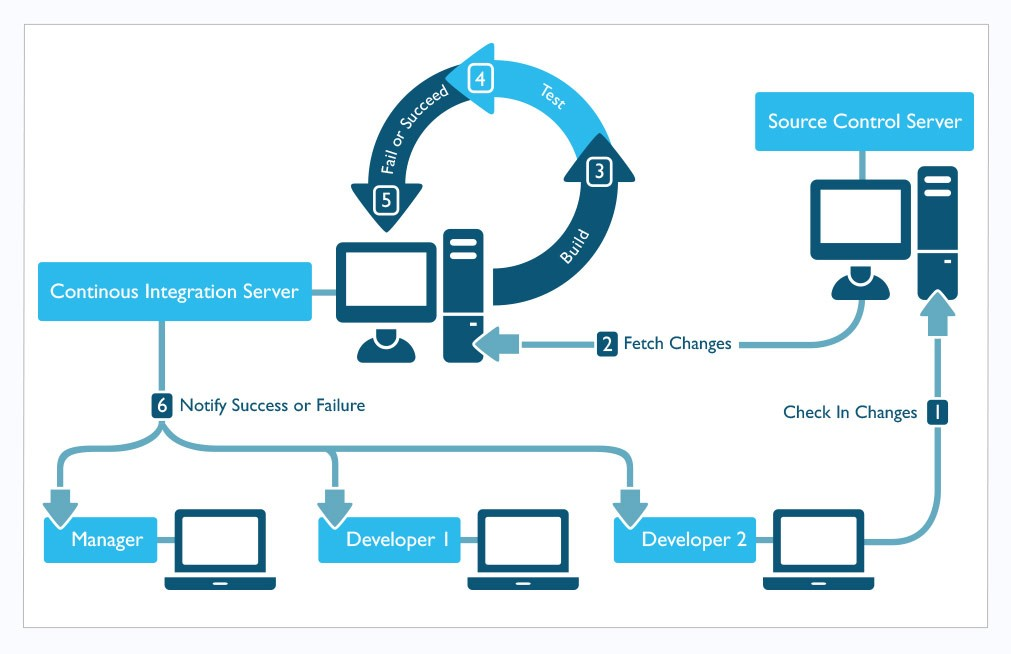
\includegraphics[width=\linewidth]{content/images/continuous_integration}\
	\quelle\url{https://insights.sei.cmu.edu/devops/2015/01/continuous-integration-in-devops-1.html}
	\caption[Continuous Integration]{Continuous Integration\\}
	\label{fig:ContinuousIntegration}  
\end{figure}
\newpage
Wie in Abbildung \ref{fig:ContinuousIntegration} \nameref{fig:ContinuousIntegration} zu erkennen ist, sorgt ein zentraler "'Continuous Integration Server"' für das Bauen und Testen der Software und informiert die zuständigen Entwickler über den Status. In der Regel wird dies bei jeder Code Änderung durchgeführt, sodass direkt erkannt wird, ob eine Änderung des Codes zu einem Erfolg oder einem Fehlschlag führt.

\begin{quote}
	"'The concept of Continuous Integration (CI) was a first step that significantly sped up the lifecycle of a product, pushing developers to commit/integrate more frequently to a shared repository, triggering automated unit-tests after each commit; as direct consequence, this helped to detect problems richt after a bad commit and reduced the necessity of back-tracking to individuate the issue in changes happend far away in time."'\cite[in Introduction]{IEEE:CDMitJenkins}
\end{quote}
Continuous Delivery ist eine natürliche Erweiterung von Continuous Integration. Trotzdem unterscheiden sich die beiden Begriffe nicht wirklich von einander. Während bei der Continuous Integration wert darauf gelegt wird, Software möglichst Fehlerfrei zu erzeugen, wird bei Continuous Delivery  darauf wert gelegt, Software möglichst regelmäßig zu deployen. Continuous Delivery beinhaltet Continuous Integration und erweitert diese um das ausliefern.

\section{Continuous Delivery Pipeline}
\label{sec:Continuous Delivery Pipeline}
Es wurden bisher die Vorteile von Continuous Delivery erläutert, wie funktioniert jedoch Continuous Delivery im einzelnen? Die einzelnen Schritte werden durch die \textit{Continuous Delivery Pipeline} beschrieben. Dabei wird der Durchlauf der Pipeline automatisch durchgeführt. Die Continuous Delivery Pipeline integriert zum einen
Die Folgende Abbildung zeigt eine mögliche Pipeline. Das Deployen in die Produktionsumgebungen "'PRODBLUE"' und "'PRODGREEN"' muss in diesem Beispiel jedoch manuel, durch klicken auf Trigger, erfolgen.

\begin{figure}[htb]
    \centering 
    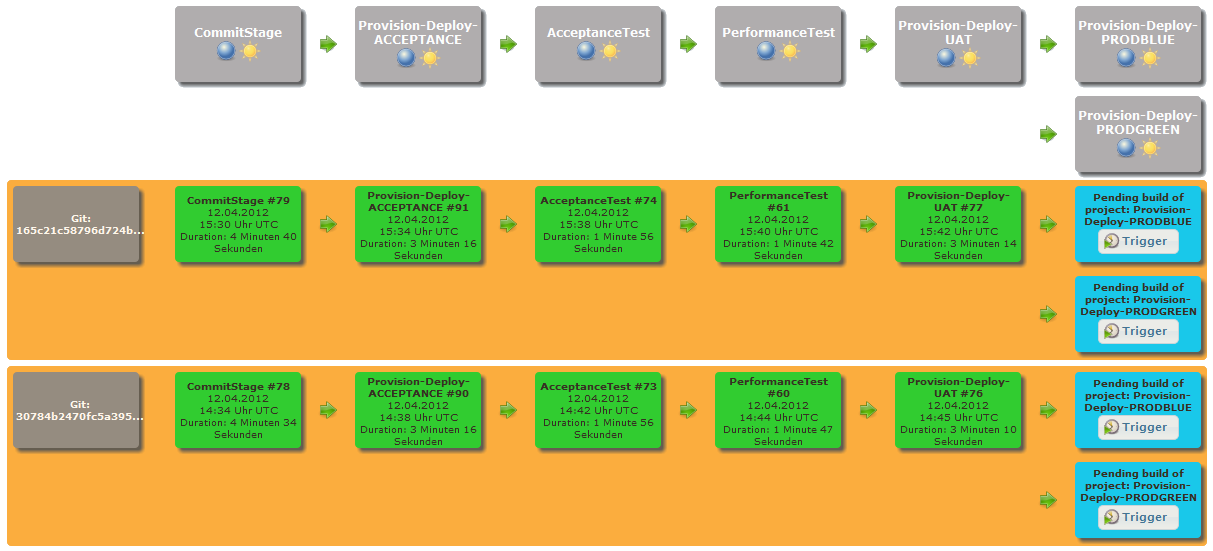
\includegraphics[width=\linewidth]{content/images/pipeline}\
    \quelle\url{https://blog.codecentric.de/en/2012/04/continuous-delivery-in-the-cloud-part1-overview/}
    \caption[Continuous Delivery Pipeline]{Continuous Delivery Pipeline\\}
    \label{fig:ContinuousDeliveryPipeline}  
\end{figure}\noindent 
Wie man in der Abbildung sehen kann beinhaltet die Pipeline alle nötigen schritte, welche zuvor in \nameref{sec:ContinuousIntegration} besprochen wurden. Hier sei noch einmal erwähnt, dass Continuous Integration alle Prozesse, bis auf den letzten (das Deployment), beinhaltet. Continuous Integration und Delivery unterscheiden sich, wie schon zu vor erwähnt, nur beim letzten Schritt, dem Deployen. Dieser wird jedoch bei Continuous Delivery Manuel ausgeführt. Unter ausgeführt ist hierbei zu verstehen, dass ein Prozess, hier durch einen klick, gestartet wird, welcher die Software, bzw. das Artefakt, automatisch in die Produktion bringt.

\section{Werkzeuge für Continuous Delivery}
\label{sec:WerkzeugeCD}
Es wurde bisher erläutert was Continuous Delivery ist, welches Vorteile es hat und welche Voraussetzungen gegeben sein müssen, damit Continuous Delivery eingeführt werden kann. Es wurde ebenfalls mit Abschnitt \ref{sec:ContinuousIntegration} \nameref{sec:ContinuousIntegration} und Abbildung \ref{fig:ContinuousIntegration} \nameref{fig:ContinuousIntegration} der Begriff \textit{Continuous Integration Server} eingeführt. Es wurde jedoch noch nicht geklärt was dieser Server genau ist und welche konkreten Aufgaben dieser besitzt. Dies soll in diesem Abschnitt geklärt werden. Zudem sollen weitere Werkzeuge vorgestellt werden, der für den \textit{Continuous Delivery Prozess} nützlich sein können. Es soll jedoch nicht die konkrete Funktionsweise von Werkzeugen erläutert werden. Einige Werkzeuge werden zum besseren Verständnis genauer erklärt als andere.
Es sei hier erwähnt, dass nicht alle Werkzeuge eingesetzt werden müssen, damit \textit{Continuous Delivery} durchgeführt werden kann, jedoch können die Werkzeuge den Prozess vereinfachen.

\subsubsection*{Continous Integration Server: Jenkins}
Der Begriff \textit{Continuous Integration} wurde bereits genau erläutert. Ein \textit{Continuous Delivery Server} ist nichts anderes, als eine Applikation die auf einem Server läuft, welche die nötigen Teilprozesse von \textit{Continuous Integration} ausführt. Wird noch einmal die Abbildung \ref{fig:ContinuousIntegration} \nameref{fig:ContinuousIntegration} betrachtet, ist der Server, auf dem die Applikation läuft, direkt neben der Box, in der "Continuous Integration Server" steht abgebildet. Ein Beispiel "Continuous Integration Server" könnte \textit{Jenkins} sein. \textit{Jenkins} ist ein sogenanntes "'Build and Management"' Werkzeug.

\begin{quote}
	"'Jenkins is an Open Source (OSS) CI Platform, whose initial objective has been the automation of the  and test process. The build system is completely written in Java and is easily extensible thanks to its plugins architecture and to extension points left into its object model. this makes of jenkins a highly customizable and flexible tool, able to cover many possible scenarios and requirements thatnks to thousands of plugins developed by its huge Open Source Community."'\cite{IEEE:CDMitJenkins}
\end{quote}
Ein "'Continuous Integration Server"'  wie \textit{Jenkins} ist die zentrale applikation, wenn es um \textit{Continuous Integration/Delivery} geht.
\begin{quote}
	"'[..] If CI startet as automation of the development phase only, pretty soon the revolution embraced the test-phase of the QA team and the deployment into various envirnment of the Ops team, involving the whole lifecycle of a product and introducing a new concept: Continuous Delivery (CD)"'\cite{IEEE:CDMitJenkins}
\end{quote}
\textit{Jenkins} hat dafür gesorgt, dass \textit{Continuous Delivery} leichter wurde. Mit der Applikation war es nun möglich, in wenigen Schritten eine eigene \textit{Continuous Delivery Pipeline} aufzubauen.

\subsubsection*{Build-Management-Tool}
\textit{Build-Management-Tool}, nicht zu verwechsel mit einem "'Build and Management"' Werkzeug, dient in erster Linie dazu, das bauen einer Software zu standardisieren. Einige bekannte Vertreter für Java sind: Maven, Ant, Gradle. Jeder dieser drei \textit{Build-Management-Tools} arbeitet auf Basis einer zentralen Datei in der die Anweisungen stehen, wie die Software gebaut werden soll. Das beinhaltet unter anderem die nötigen Abhängigkeiten (auch Dependency-Management genannt), sowie die Pfade zu den Dateien, welche zusätzlich eingebunden werden sollen.
\\\\
Durch \textit{Build-Management-Tools} können zudem zusätzliche Aktionen durchgeführt werden, wie zum Beispiel das ausführen von Unit-Tests, sowie die Steuerung darüber, was bei fehlgeschlagenen Tests passieren soll.
\\\\
Unter anderem nutzt \textit{Jenkins} solche \textit{Build-Management-Tools} zum bauen der jeweiligen Projekte.

\subsubsection*{Automatischer Aufbau der Infrastruktur}
Nachdem Werkzeuge eingeführt worden sind, mit deren Hilfe standardisierte Software innerhalb und außerhalb von \textit{Continuous Integration}, gebaut werden kann. Muss, damit \textit{Continuous Delivery} durchgeführt und ebenfalls standardisiert werden kann, eine bzw. zwei neue Werkzeuge eingeführt werden.
\\\\
Damit Software automatisch, im Rahmen von \textit{Continuous Delivery}, ausgeliefert werden kann, muss neben den Tests auch das aufbauen der Infrastruktur automatisiert werden. Zwei Werkzeuge um dies zu erreichen sind \textit{Chef} und \textit{Puppet}.
\begin{quote}
	"'Puppet and Chef are the most commonly used IT Automation Tools used by DevOps to set up the infrastructure, speeding up the process of installing the required software, moddleware and various dependencies."'\cite{IEEE:CDMitJenkins}
\end{quote}
Damit Software ohne Probleme automatisch deployed werden kann, müssen ggf. Änderungen an der Infrastruktur durchgeführt werden bzw. eine neue Infrastruktur aufgesetzt werden. Letzteres ist zum Beispiel bei der Skalierung notwendig. Damit jede Instanz gleich, bzw. jede Änderung der vorhandenen Instanzen nachvollzogen werden kann, müssen alle Schritte dokumentiert werden. Die technische Dokumentation geschieht mit Hilfe von \textit{Chef/Puppet}. Nach dieser Dokumentation kann das jeweilige Werkzeug gestartet werden und eine standardisierte Infrastruktur wird aufgebaut.

\subsubsection*{Binary Repository Manager}
Zuletzt muss noch eine Möglichkeit gefunden werden, um die einzelnen Versionen von Artefakten zu Versionieren und sicher zu lagern. Hier können sogenannte \textit{Binary Repository Manager} eingestzt werden.

\begin{quote}
    "'It’s a single gateway through which you access external artifacts, and store your own build artifacts. By centralizing the management of all binary artifacts, it overcomes the complexity arising from the diversity of binary types, their position in the workflow and the dependencies between them."'\cite{BRM}
\end{quote}

In Zusammenarbeit mit \textit{Build-Management-Tools}, kann eine sichere und einfache Möglichkeit des \textit{Dependency Managements} aufgebaut werden.
\\\\
Nachdem die \textit{Continuous Delivery Pipeline} durchlaufen wurde und alle Tests erfolgreich bestanden wurden, wird das Artefakt im \textit{Binary Repository Manager} gespeichert.

\section{Einführung von Continuous Delivery}
\label{sec:EinfuehrungCD}
In Kapitel \ref{sec:problemstellung} \nameref{sec:problemstellung} wurden bereits zwei Fälle beschrieben, in denen kein Continuous Delivery eingesetzt wurde. Darauf aufbauend wird nun Schritt für Schritt der bestehende Entwicklungsprozess, des fiktive Beispiels von Eberhard Wolff, zu Continuous Delivery überführt. Für die Erstellung der \textit{Continuous Delivery Pipeline} werden die zuvor erläuterten Werkzeuge eingesetzt. Des besseren Verständnis wegen, wird davon ausgegangen, dass in der Programmiersprache Java programmiert wird. Außerdem wird davon ausgegangen, dass eine Versionsverwaltung wie \textit{Git} eingesetzt wird, um Code-Änderungen zu verwalten und nach zu vollziehen.
\\\\
Bevor eine \textit{Continuous Delivery Pipeline} aufgebaut werden kann, muss zunächst einmal geklärt werden, welche Ziele erreicht werden sollen. Eines der Hauptziele ist es den Deployment-Prozess zu verkürzen. Anstatt nur einmal im Monat zu deployen, soll langfristig gesehen, so oft wie möglich deployed werden. Im Zuge dessen, ist das nächste Hauptziel, die Qualitätssicherung zu verbessern, in dem Tests nicht mehr manuell ausgeführt werden, sondern innerhalb der \textit{Continuous Delivery Pipeline} automatisch ausgeführt werden.

Als ersten Schritt wird ein \textit{Continuous Integration Server} aufgesetzt. Dafür wird das bereits erwähnte Werkzeug \textit{Jenkins} eingesetzt. Jenkins wird zunächst dafür verwende, die in Abbildung \ref{fig:ContinuousIntegration} \nameref{fig:ContinuousIntegration} gezeigten Prozesse, abzubilden. Mit diesem Schritt wird die "'Commit Stage"' abgebildet.

\begin{quote}
    "'The goal of the commit stage is to compile the source code written by the development teams into executable binaries."'\cite{CD:AutomatedTesting}
\end{quote}

Jenkins wird dabei so eingestellt, dass bei jeder Code-Änderung in der Versionsverwaltung dieser Prozess durchlaufen wird. Damit ist der Anfang der \textit{Continuous Delivery Pipeline} aufgebaut und kann durchlaufen werden.
\\\\
Damit die aus dem ersten Schritt entstehende Artefakt gespeichert und wiederverwendet werden können wird ein zentrales \textit{Binary Repository Manager} wie Nexus oder Artifactory aufgesetzt. Damit wird, wie schon im Abschnitt \ref{sec:WerkzeugeCD} \nameref{sec:WerkzeugeCD} erläutert, sichergestellt, dass alle Versionen eines Artefaktes archiviert werden und durch andere Projekte wiederverwendet werden können. Damit dies geschieht, muss Jenkins noch so eingestellt werden, dass nach einem erfolgreichen durchlaufen der \textit{Pipeline}, das entstandene Artefakt in das zentrale \textit{Binary Repository Manager} archiviert wird.
\\\\
Als nächsten Schritt wird das Softwareprojekt um ein \textit{Build-Management-Tool} wie Maven erweitert. Mit diesem Schritt soll sichergestellt werden, dass die Software nach einem standardisierten Verfahren gebaut wird, wodurch bei mehrmaligen ausführen der Commit Stage, stets das selbe Resultat erwartet werden kann.  Mit dem \textit{Build-Management-Tool} wird außerdem das Problem, der Abhängigkeiten gelöst. Damit ist gemeint, das mit Hilfe des Werkzeugs Abhängigkeiten zu anderen Artefakten automatisch aufgelöst werden können und nicht mehr manuell zum Projekt hinzugefügt werden müssen. Die Abhängigkeiten werden dabei aus dem zentralen \textit{Binary Repository Manager} geladen.
\newpage
Nach diesem Schritt sieht die aufgebaute Infrastruktur des Entwicklungsprozesses wie folgt aus:

\begin{figure}[htb]
    \centering 
    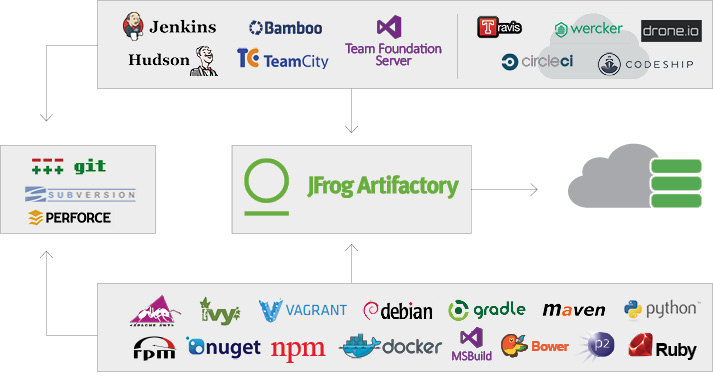
\includegraphics[width=\linewidth]{content/images/CISetup}\
    \quelle\url{https://www.jfrog.com/article/jenkinshudson/}
    \caption[Continuous Integration Setup]{Continuous Integration Setup. Oben die möglichen "`Continuous Integration Server"', links die möglichen Code-Versionsverwaltungen, unten die möglichen "`Build-management-Tools"'}
    \label{fig:CISetup}  
\end{figure}

Die Abbildung zeigt ein Continuous Integration Setup. Oben sind die möglichen "'Continuous Integration Server"'. Diese greife zum einen auf die Code-Versionsverwaltung zu, um den Code zu laden, mit dem ein Artefakt gebaut werden soll. Zum anderen speichert er das erfolgreich entstandene Artefakt mit Hilfe von Artifactory. Mit einen der unten aufgeführten Build-management-Tools können diese Artefakte in Projekte übernommen werden, ohne sie manuell hinzufügen zu müssen.
\\\\
Es wurde bisher dafür gesorgt, das Artefakte standardisiert gebaut werden können und das erfolgreiche Resultat, mit Hilfe eines \textit{Binary Repository Managers}, archiviert wird. Jedoch ist der Prozess der Überführung zu \textit{Continuous Delivery} noch nicht abgeschlossen. Ein weiterer wichtiger Schritt ist die Automatisierung der Tests. Zu nächst einmal sollten Unit-Tests geschrieben werden, die den Code Überprüfen. Zusätzlich sollten Akzeptanz Tests geschrieben werden, womit die "'Acceptance Test Stage"' abgebildet wird.

\begin{quote}
    "'The goal of the acceptance test stage to verify that the software produced in the commit stage meets the business requirements using automated tests."'\cite{CD:AutomatedTesting}
\end{quote}

Neben den Akzeptanz Test, sollten noch weitere Tests erstellt werden, wie zum Beispiel Performance Tests, auch genannt "'Capacity Tests"'. Mit diesem Schritt wurde ein weiterer Schritt, der \textit{Continuous Delivery Pipeline} hinzugefügt.

\begin{quote}
    "'The goal of the capacity test stage is to make sure that the capacity requirements of the software are met. this stage also includes tests for scalability and endurance"'\cite{CD:AutomatedTesting}
\end{quote}

Mit Hilfe von Jenkins können diese Tests automatisch, innerhalb der \textit{Continuous Delivery Pipeline} durchlaufen werden.
\\\\
Es können noch weitere Schritte wie zum Beispiel Oberflächen Tests durchgeführt werden. Oft ist es dabei nötig das Artefakt in eine Tests Umgebung zu deployen. Dabei können mit Hilfe von Chef/Puppet ganze Systeme innerhalb der Pipeline aufgebaut werden. Somit kann zum Beispiel eine ganze Produktiv Infrastruktur, nur zum Testen, nachgebaut werden. Hierbei sei jedoch zu beachten, dass das Produktiv System nicht zu groß sein sollte, da der Prozess der Infrastruktur Erstellung zu lange dauern würde.
\\\\
Es wurden jetzt alle Wichtigen Schritte durchgeführt, die das Bauen und Testen abbilden. Die dadurch entstandene \textit{Continuous Delivery Pipeline} wird, sobald eine Code-Änderung durchgeführt wurde, komplett durchlaufen. Entsteht in einem Schritt ein Problem, wird die Pipeline abgebrochen und der Entwickler erhält eine direkte Rückmeldung über den Fehler. Wird hingegen die Pipeline ohne weitere Probleme durchlaufen, wird das entstandene Artefakt in einem \textit{Repository Manager} archiviert. Abschließend kann unter anderem der Deployment-Prozess ebenfalls automatisiert werden und bei jedem erfolgreichen Durchlauf durchgeführt werden. Der Deployment-Prozess kann jedoch auch soweit automatisiert werden, das mit einem klick das Artefakt ausgeliefert wird, jedoch nicht nach jedem erfolgreichen Durchlauf der Pipeline ausgeführt wird.
\\\\
Abschließend sei noch erwähnt, dass es nicht nötig ist, von "`alle vier Wochen"' zu "`wann immer man möchte"' , über Nacht zu springen.

Steve nelly und Steve Stolt von Rally Software schreiben dazu folgendes\cite{RallySofware2013} :
\begin{quote}
    "'Jumping directly from [four] week releases to a pus-to-production strategy is clearly not a sensible approach. We began by shrinking our release cycles down to fortnightly, weekly, semiweekly and finally at-will. These steps took weeks or even monts of preparatory work to get our deploy process streamlined and automated"'\cite[You do not have to go from eight to zero overnight]{RallySofware2013}
\end{quote}